\chapter{Výsledky}
Pro zhodnocení výsledků našeho vyhledávače jsme provedli dva druhy testů. V
rámci prvního jsme porovnávali výsledky našeho vyhledávače s ostatními veřejně
dostupnými vyhledávači spojení. V druhém testu jsme na pevně dané trase a času
zkoumali, jaký vliv na nalezené trasy má různé nastavení penalt a rychlostí
chůze. Aplikaci jsme také profilovali, abychom zjistili, v jakých částech se
tráví nejvíce času a měly by se optimalizovat jako první.

\section{Porovnání s jinými vyhledávači}
Výsledky našeho vyhledávače jsme porovnávali s veřejně dostupnými vyhledávači
spojení po Praze: IDOS\footnote{\url{http://idos.cz}},
Mapy.cz\footnote{\url{http://mapy.cz}} a Google
Maps\footnote{\url{http://maps.google.com}}. 

IDOS je nejstarší a nejznámější vyhledávač spojení. Jako jediný z vyhledávačů
nepodporuje hledání pěších tras, vyhledává pouze v jízdních řádech, přestupy
mezi zastávkami řeší pomocí tabulky, která obsahuje dvojice zastávek a čas
přesunu mezi nimi. Jako vstup je možné zadat adresu, ale vyhledávač nalezne
pouze nejbližší zastávky podle vzdušné vzdálenosti a hledá z nich / do nich. 
Na druhou stranu umožňuje široké možnosti nastavení vyhledávání spojů -- volbu
minimálních časů na přestup, typů dopravních prostředků, počtu přestupů, \dots

Mapy.cz a Google Maps jsou původně mapové služby, které do svých vyhledávačů
přidaly možnost vyhledávání kromě pěších cest i spojení MHD. Protože se jedná
primárně o mapové služby, vyhledávače neumožňují žádné (Mapy.cz) nebo jen velmi
omezené (Google Maps) přizpůsobení. 

Při porovnávání vyhledaných spojení jsme všude nechali výchozí nastavení a náš
vyhledávač jsme nastavili tak, jak si myslíme, že jsou nastaveny ostatní
vyhledávače, aby byly výsledky porovnatelné. Konkrétní nastavení je výchozí
nastavení {\tt config/speeds.yaml} v příloze. Přestupy nebyly nijak
penalizovány, na zastávce bylo nutné mít aspoň 30\,s čas mezi příchodem /
příjezdem a odjezdem.

Testovali jsme následující trasy, které známe i z reálného provozu. Jednotlivé
trasy zkoumaly různé aspekty vyhledávačů:
\begin{itemize}
	\item {\em Kolej 17. listopadu -- Přírodovědecká fakulta UK, Albertov}\\ Tato
	cesta je zaměřena na obtížnou dopravní situaci okolo kolejí 17.
	listopadu. Spojení na Nádraží Holešovice je nejspolehlivější pěšky,
	autobus 201 většinou nejede dle jízdního řádu. V případě cesty tramvají
	č. 17 je možné jednak využít od kolejí autobus 112, ovšem s výstupem na
	Povltavské, nikoli na Trojské, případně dojít přímo na Trojskou pěšky.
	Všechny tyto možnosti dávají smysl při hledání cesty na Albertov. Na
	durhém konci také není situace přímočará, při cestě od metra je dobrou
	alternativou jít pěšky z Vyšehradu. 
	\item {\em Kolej 17. listopadu -- Čistírna odpadních vod, Bubeneč}\\ Tato
	cesta zkoumá schopnosti pěší navigace, protože jednou z možností je jít
	pěšky přes Stromovku. Také je zde vidět rozdíl mezi naším vyhledávačem a
	Google Maps na jedné straně a IDOSem a Mapy.cz na straně druhé, které
	využívají znalosti jízdních řádů integrovaných vlaků a umí je na této
	cestě využít.
	\item {\em Kovanecká -- Gymnázium Omská}\\ Tato cesta opět zkoumá schopnost
	využívat delší pěší přesuny a také dávat přednost časově kratším cestám
	s přestupy. 
	\item {\em FEL ČVUT, Dejvice -- Hlávkova kolej}\\ Tato cesta je zaměřena na
	hledání aktuálně nejrychlejší alternativy z několika rovnocenných. Dobré
	alternativy nevyžadují dlouhé pěší přesuny.
\end{itemize}
\subsection{Kolej 17.\,listopadu -- Albertov}

Vyhledávač IDOS našel následující spojení

\begin{tabular}{|l|c|c|r|}\hline
{\bf Zastávka}&{\bf Příjezd}&{\bf Odjezd}&{\bf Linka}\\\hline
Kuchyňka&&13:23&201\\\hline
Bulovka&13:26&13:28&24\\\hline
Albertov&14:04&&\\\hline
\end{tabular} 

\begin{tabular}{|l|c|c|r|}\hline
{\bf Zastávka}&{\bf Příjezd}&{\bf Odjezd}&{\bf Linka}\\\hline
Kuchyňka&&13:25&201\\\hline
Nádraží Holešovice&13:28&13:32&C\\\hline
Florenc&13:36&13:41&B\\\hline
Karlovo náměstí&13:47&&\\\hline
Palackého náměstí&&13:52&18\\\hline
Albertov&13:56&&\\\hline
\end{tabular} 

\begin{tabular}{|l|c|c|r|}\hline
{\bf Zastávka}&{\bf Příjezd}&{\bf Odjezd}&{\bf Linka}\\\hline
Pelc Tyrolka&&13:26&112\\\hline
Trojská&13:29&13:33&17\\\hline
Výtoň&13:54&13:57&14\\\hline
Albertov&13:59&&\\\hline
\end{tabular} 

\begin{figure}[h]
  \centering
    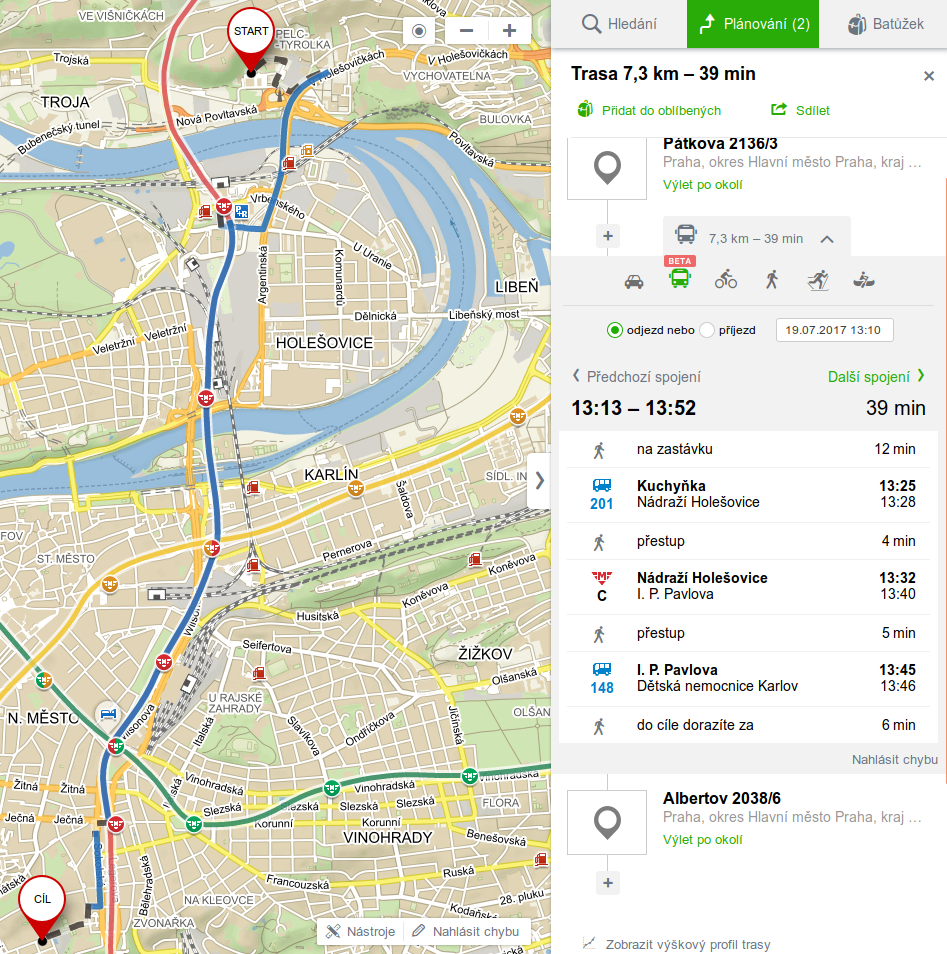
\includegraphics[width=\textwidth]{../img/kolej-albertov-seznam.png}
  \caption{Spojení Kolej 17. listopadu -- Albertov podle Mapy.cz}
  \label{fig:kolej-albertov-seznam}
\end{figure}
\begin{figure}[h]
  \centering
    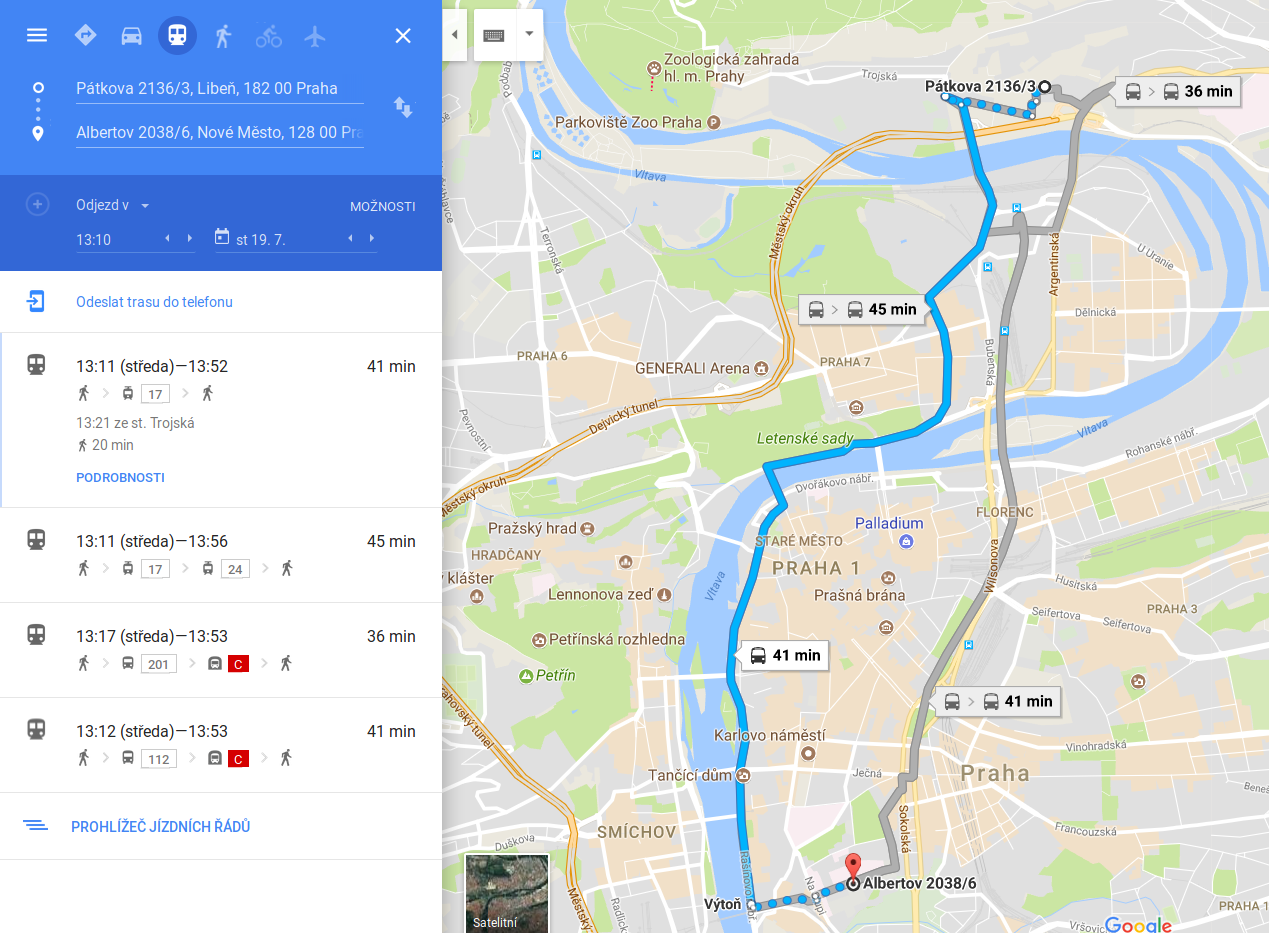
\includegraphics[width=\textwidth]{../img/kolej-albertov-google.png}
  \caption{Spojení Kolej 17. listopadu -- Albertov podle Google Maps}
  \label{fig:kolej-albertov-google}
\end{figure}

\subsection{Kolej 17.\,listopadu -- Čistírna odpadních vod}
Vyhledávač IDOS našel následující spojení:

\begin{tabular}{|l|c|c|r|}\hline
{\bf Zastávka}&{\bf Příjezd}&{\bf Odjezd}&{\bf Linka}\\\hline
Kuchyňka&&13:25&201\\\hline
Nádraží Holešovice&13:28&13:45&Os 10440\\\hline
Praha-Podbaba&13:49&&\\\hline
\end{tabular} 

\begin{tabular}{|l|c|c|r|}\hline
{\bf Zastávka}&{\bf Příjezd}&{\bf Odjezd}&{\bf Linka}\\\hline
Pelc Tyrolka&&13:26&112\\\hline
Trojská&13:29&13:33&17\\\hline
Nádraží Holešovice&13:35&13:45&Os 10440\\\hline
Praha-Podbaba&13:49&&\\\hline
\end{tabular} 

\begin{figure}[h]
  \centering
    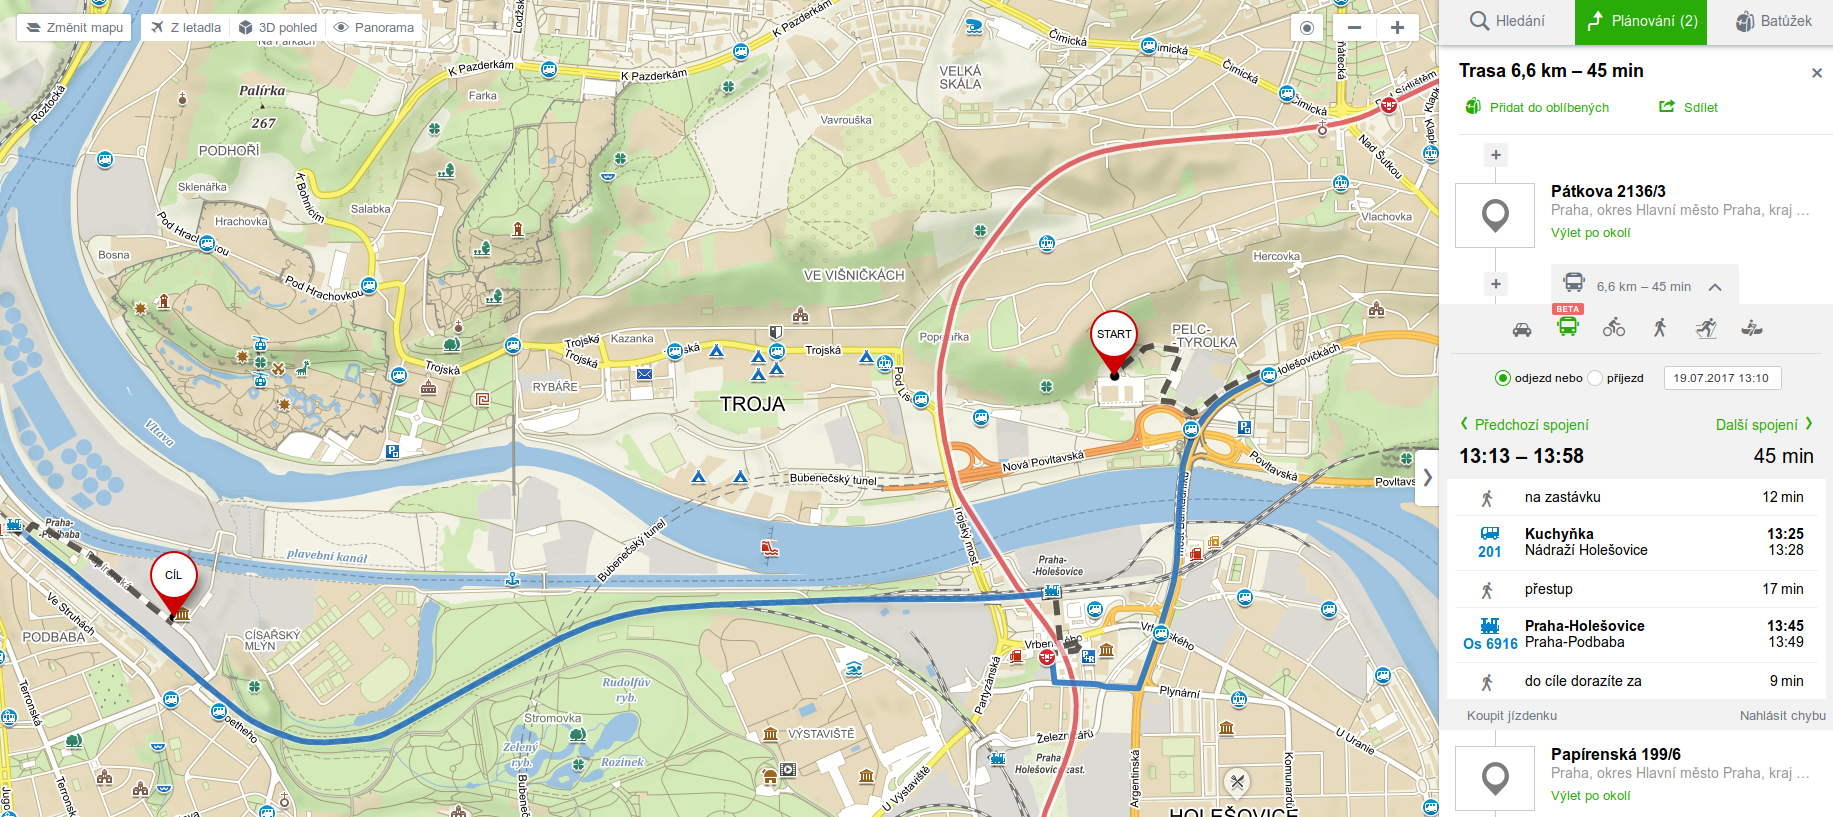
\includegraphics[width=\textwidth]{../img/kolej-bubenec-seznam.png}
  \caption{Spojení Kolej 17. listopadu -- Čistírna odpadních vod podle Mapy.cz}
  \label{fig:kolej-bubenec-seznam}
\end{figure}
\begin{figure}[h]
  \centering
    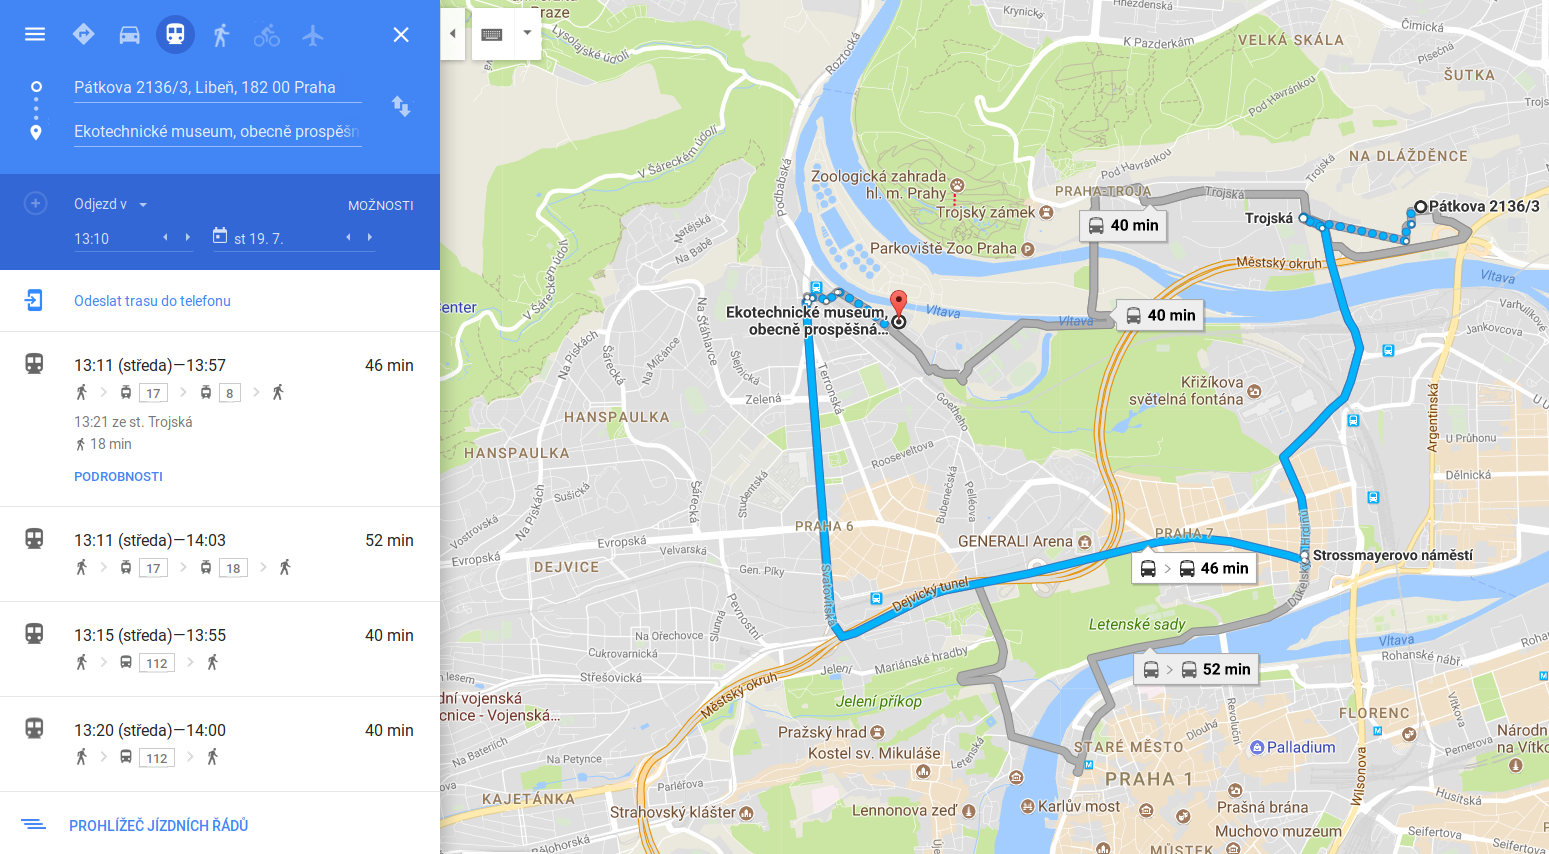
\includegraphics[width=\textwidth]{../img/kolej-bubenec-google.png}
  \caption{Spojení Kolej 17. listopadu -- Čistírna odpadních vod podle Google
  Maps}
  \label{fig:kolej-bubenec-google}
\end{figure}

\subsection{Kovanecká -- Gymnázium Omská}
Vyhledávač IDOS našel tato spojení:

\begin{tabular}{|l|c|c|r|}\hline
{\bf Zastávka}&{\bf Příjezd}&{\bf Odjezd}&{\bf Linka}\\\hline
Balabenka&&13:20&6\\\hline
Kubánské náměstí&14:11&&\\\hline
\end{tabular} 

\begin{tabular}{|l|c|c|r|}\hline
{\bf Zastávka}&{\bf Příjezd}&{\bf Odjezd}&{\bf Linka}\\\hline
Divadlo Gong&&13:21&16\\\hline
Želivského&13:35&13:41&150\\\hline
Slavia&13:46&13:52&22\\\hline
Kubánské náměstí&13:53&&\\\hline
\end{tabular} 
\begin{figure}[h]
  \centering
    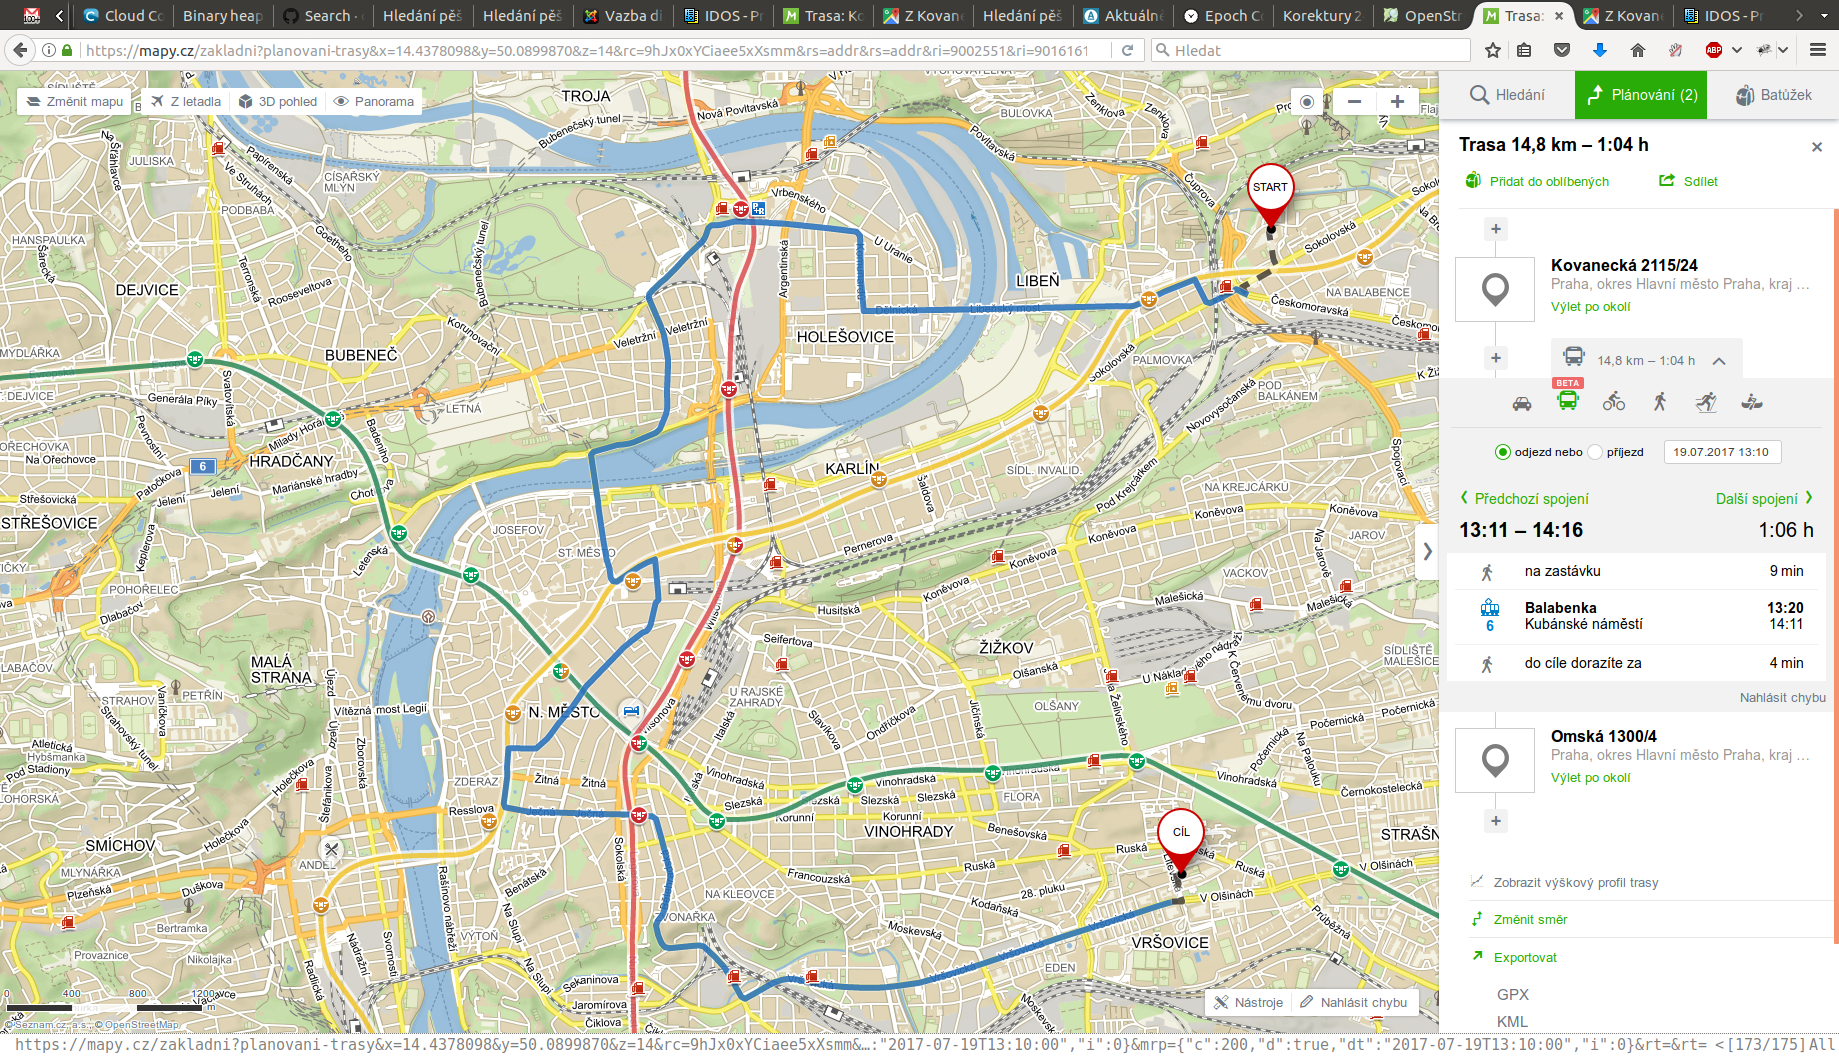
\includegraphics[width=\textwidth]{../img/kovanecka-omska-seznam.png}
  \caption{Spojení Kovanecká -- Gymnázium Omská podle Mapy.cz}
  \label{fig:kovanecka-omska-seznam}
\end{figure}
\begin{figure}[h]
  \centering
    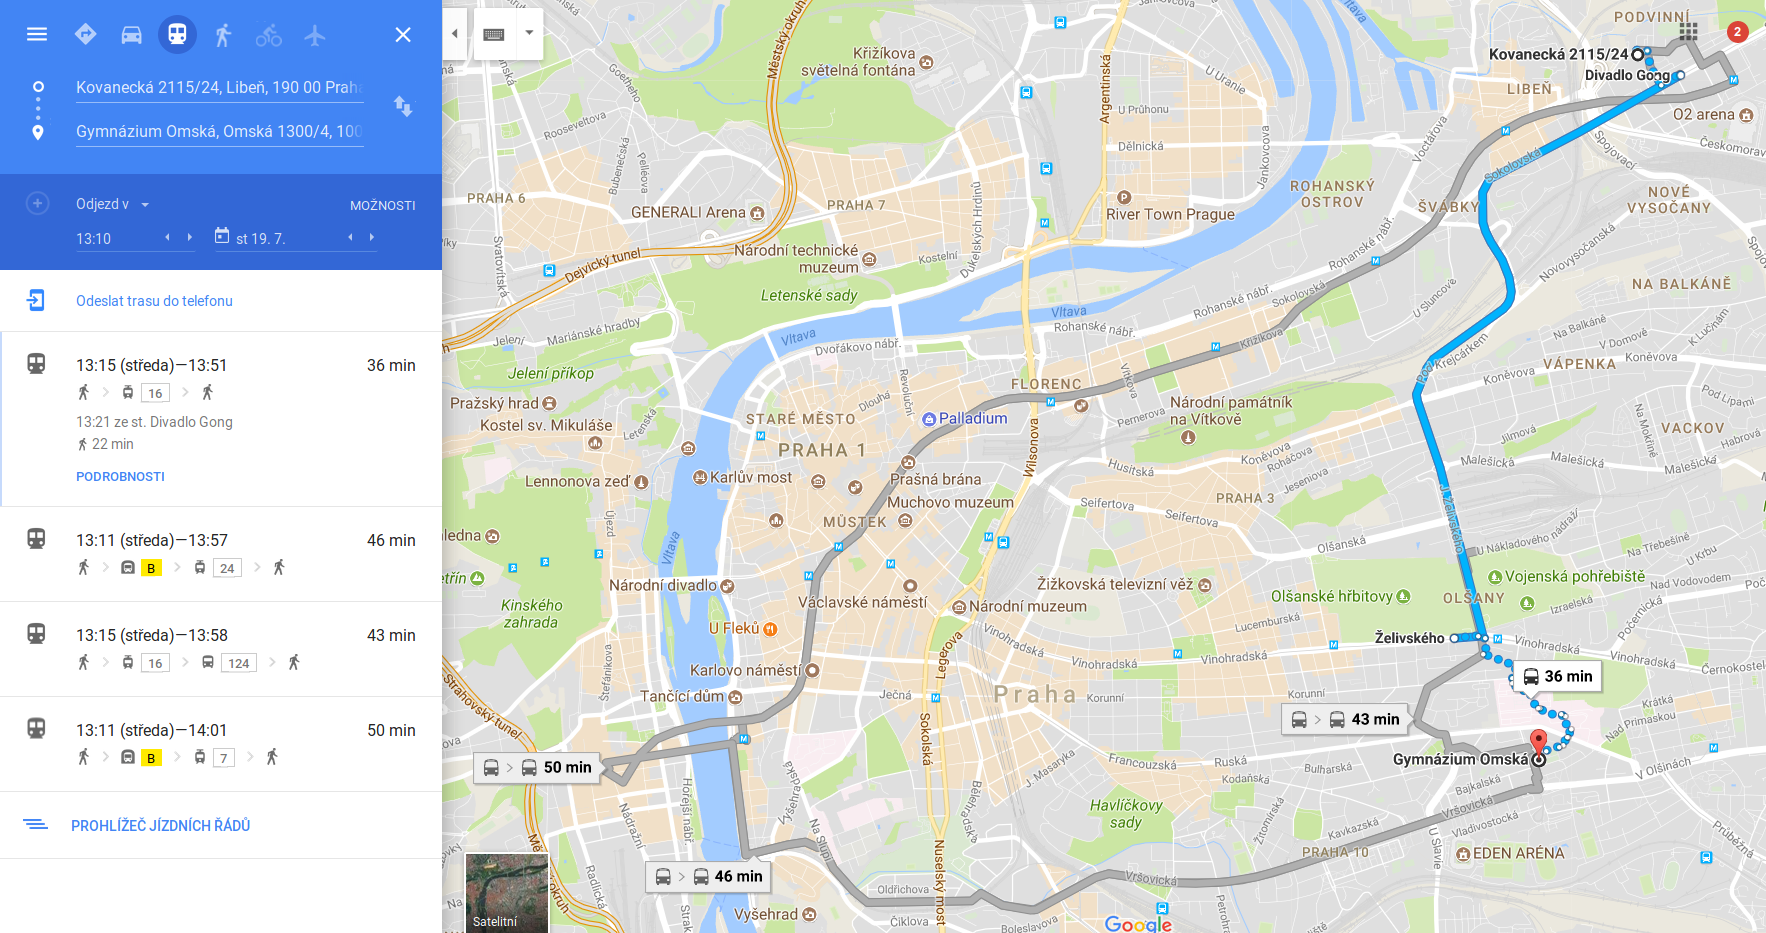
\includegraphics[width=\textwidth]{../img/kovanecka-omska-google.png}
  \caption{Spojení Kovanecká -- Gymnázium Omská podle Google Maps}
  \label{fig:kovanecka-omska-google}
\end{figure}

\subsection{FEL ČVUT -- Hlávkova kolej}
Vyhledávač IDOS našel tato spojení:

\begin{tabular}{|l|c|c|r|}\hline
{\bf Zastávka}&{\bf Příjezd}&{\bf Odjezd}&{\bf Linka}\\\hline
Dejvická&&13:16&A\\\hline
Můstek&13:22&13:29&B\\\hline
Karlovo náměstí&13:32&&\\\hline
\end{tabular} 

\begin{tabular}{|l|c|c|r|}\hline
{\bf Zastávka}&{\bf Příjezd}&{\bf Odjezd}&{\bf Linka}\\\hline
Vítězné náměstí&&13:19&18\\\hline
Karlovo náměstí&13:37&&\\\hline
\end{tabular} 

\begin{tabular}{|l|c|c|r|}\hline
{\bf Zastávka}&{\bf Příjezd}&{\bf Odjezd}&{\bf Linka}\\\hline
Dejvická&&13:21&A\\\hline
Staroměstská&13:25&13:30&18\\\hline
Karlovo náměstí&13:37&&\\\hline
\end{tabular} 

\begin{figure}[h]
  \centering
    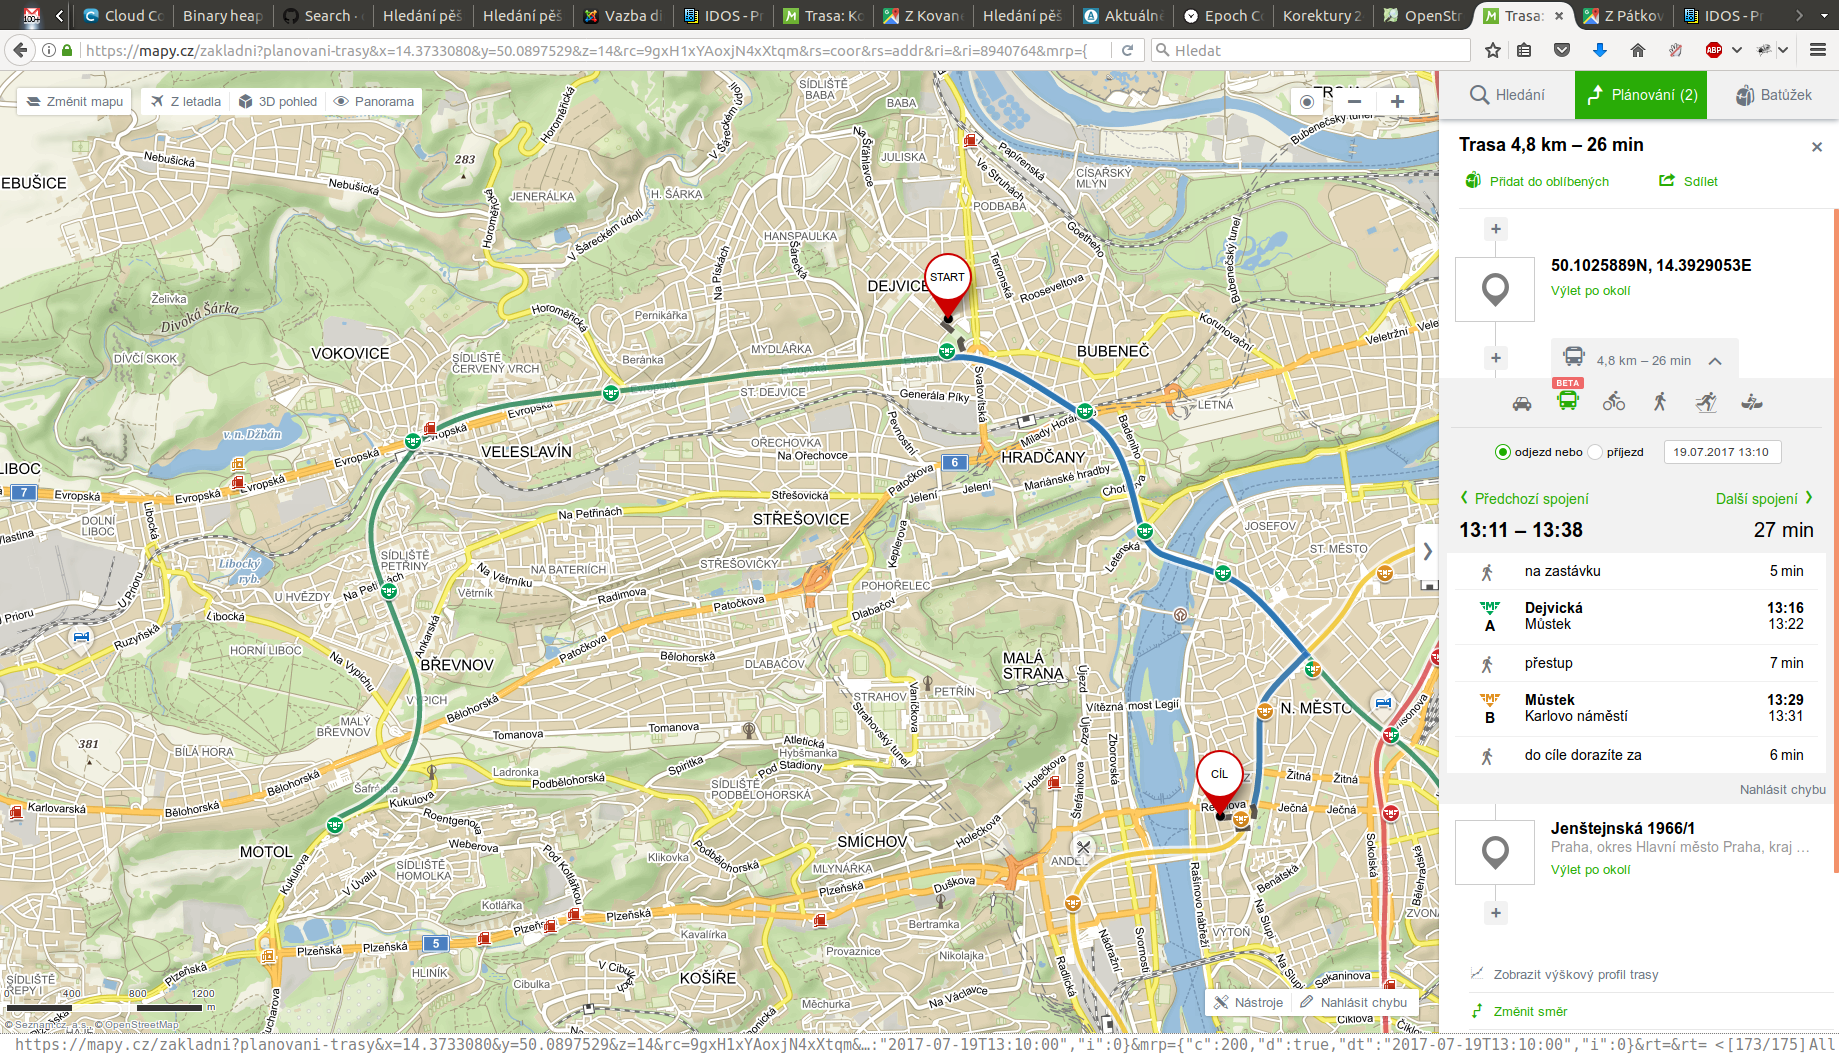
\includegraphics[width=\textwidth]{../img/fel-hlavkova-seznam.png}
  \caption{Spojení FEL ČVUT -- Hlávkova kolej podle Mapy.cz}
  \label{fig:fel-hlavkova-seznam}
\end{figure}
\begin{figure}[h]
  \centering
    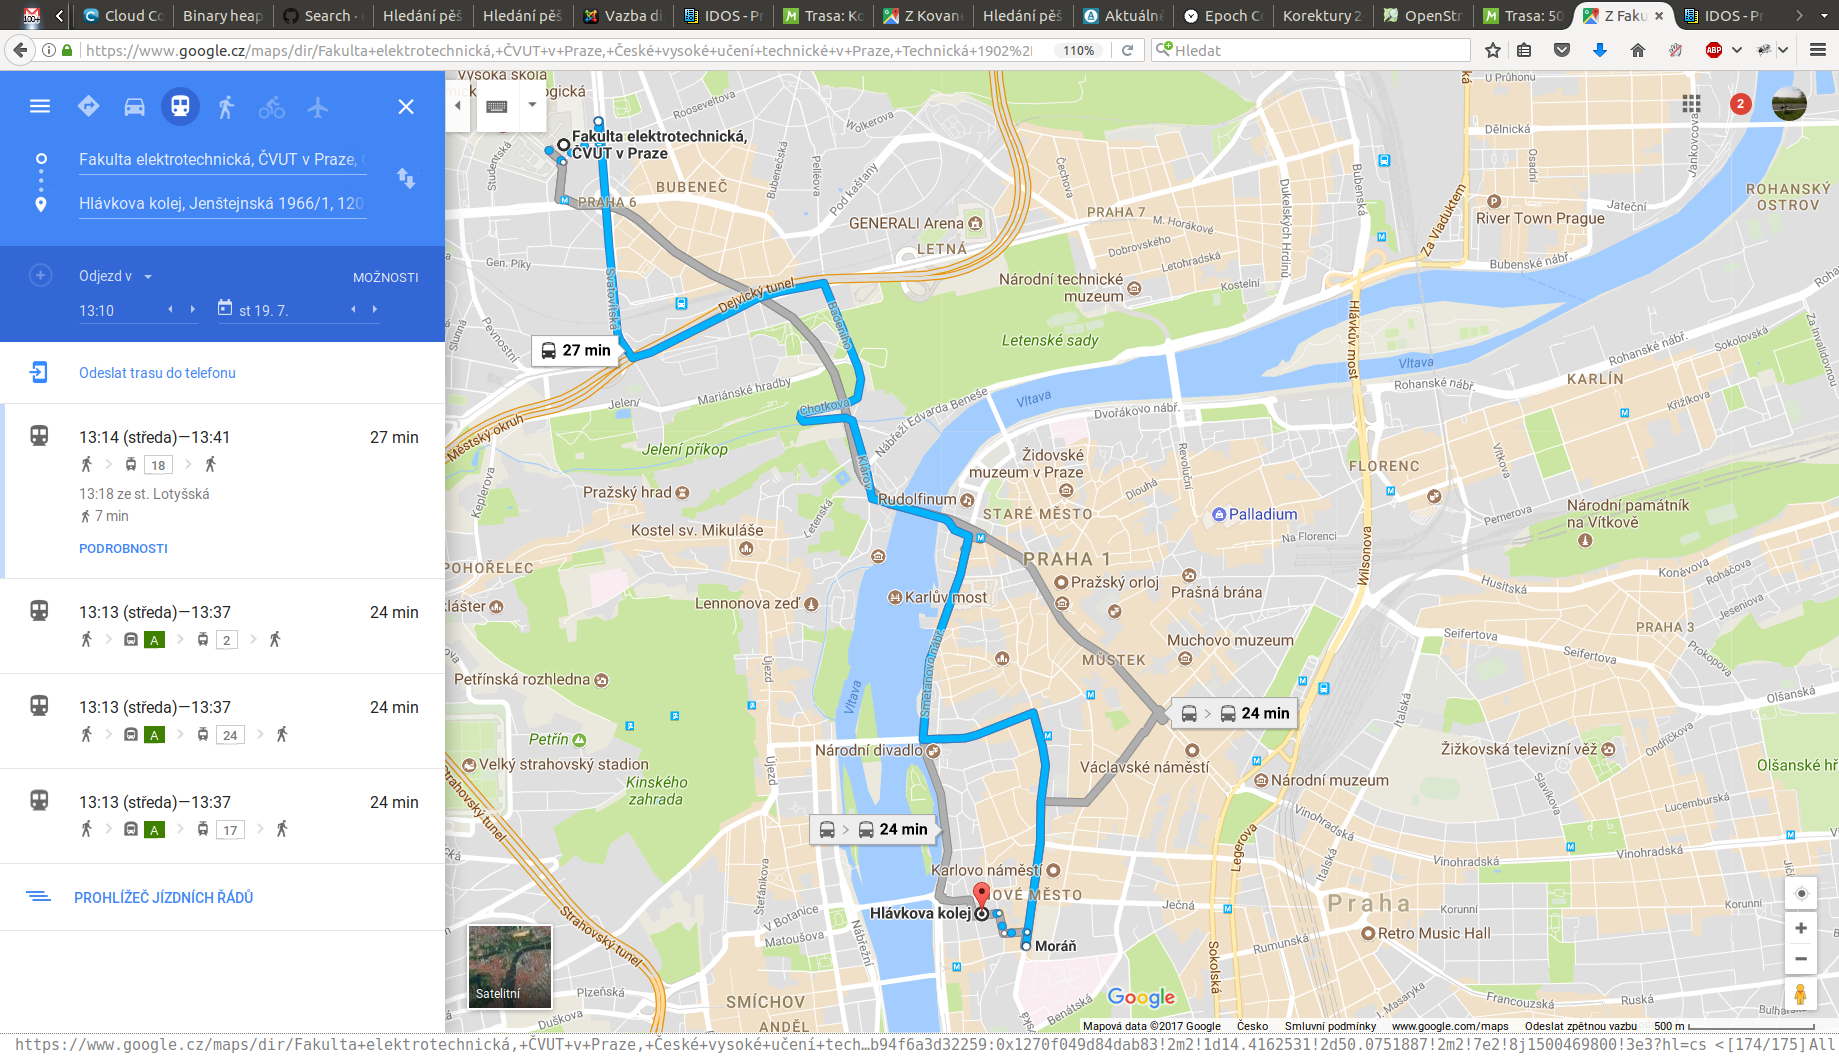
\includegraphics[width=\textwidth]{../img/fel-hlavkova-google.png}
  \caption{Spojení FEL ČVUT -- Hlávkova kolej podle Google Maps}
  \label{fig:fel-hlavkova-google}
\end{figure}
\section{Porovnání různých nastavení}
Pro porovnání různých nastavení našeho vyhledávače jsme zvolili trasu Kolej
17.listopadu -- Albertov, protože tato trasa poskytuje několik různých
alternativ spojení, tudíž jsme předpokládali, že se tyto alternativy projeví v
nalezených trasách. Všechna spojení byla hledána od stejného času, pracovní den
v brzkém odpoledni, tudíž by měl být eliminován vliv návazností, které fungují
jen v určité minuty, protože podmínky jsou pro všechna hledání stejné.

Porovnávali jsme tato nastavení:
\begin{itemize}
	\item {\em Standardní}\\Základní nastavení vyhledávače, měl by se chovat
	obdobně jako jiné webové vyhledávače
	\item {\em Bez autobusu 201}\\ Linka 201 je ve směru z kolejí na Nádraží
	Holešovice tak nespolehlivá, že je lepší s ní vůbec nepočítat. Toto
	nastavení ji pomocí penalty {\tt inf} vyřazuje z hledání.
	\item {\em Penalizace autobusů}\\ Test na penalizaci typu dopravního
	prostředku, měl by se snažit vyhýbat spojení autobusem a hledat jiné
	alternativy.
	\item {\em Jen jeden spoj}\\ Test na hledání, kterým spojem jet, pokud
	nechceme nikde přestupovat.
	\item {\em Pouze pěšky}\\ Ačkoli je vyhledávač stavěn na kombinované hledání
	pěších přesunů a cest MHD, stále by měl umět najít i pouze pěší cestu.
	\item {\em Na kole}\\ Tento test předpokládá jízdu na skládacím kole nebo
	koloběžce, tedy něčem, co lze vzít s sebou do MHD. Testuje nestandardní
	vyhledávací parametry.
	\item {\em Penalizace pěších přesunů}\\ Opak předchozího testu, snažíme se
	minimalizovat pěší přesuny a co nejvíce se pohybovat pomocí MHD.
\end{itemize}
\subsection{Standardní}
Nastavení je základní, takové, jaké se nachází v repozitáři jako {\tt
config/speeds.yaml}. U ostatních testů bude uveden pouze rozdíl oproti tomuto
nastavení.

Nalezené spojení je plně použitelné. Drobným překvapením bylo, že vyhledávač
nalezl spojení z metra Vyšehrad, což je korektní cesta, ale nebyla očekávaná.
\TODO opravit Botič a přegenerovat
\subsection{Bez autobusu 201}
Oproti standardnímu nastavení je pouze penalizace linky 201 nastavena na {\tt
inf}, tato linka by tedy k hledání vůbec neměla být použita.

Nalezené spojení využívá druhou vhodnou trasu na Albertov, která vede na tramvaj
č. 17 a tou přes centrum. Eliminuje tím potřebu cesty na Nádraží Holešovice.
Pro cestu na Trojskou vhodně využívá autobusu 112, ze kterého vystupuje na
Povltavské, odkud je to na tramvajovou zastávku Trojská jen několik desítek
metrů, na rozdíl od značně vzdálené autobusové zastávky Trojská.

\subsection{Penalizace autobusů}
Oproti standardnímu nastavení mají autobusy fixní penaltu nastavenou na 100 a za
každou sekundu v autobuse dostanou penaltu dalších 10. 

Vyhledávač pro toto nastavení nalezl dvě alternativy cesty. První je v
optimálním případě rychlá, proto je zařazena, i když autobus využívá i přes
penaltu. Protože je penalta závislá na době cestování, vyhledávač využívá
volného přestupu na Nádraží Holešovice a velí vystoupit už na zastávce
Jankovcova, odkud se stihne dojít pěšky na stejné metro, jako by se stihlo
autobusem a ušetří se penalta za čas. Druhá varianta je podobná předchozímu
hledání, ale z důvodu penalizace autobusů je pro cestu na Trojskou zvolena pěší
chůze. Vzhledem k velké časové rezervě na Trojské oba způsoby dopravy stihnou
stejnou tramvaj a tudíž je kvůli vysoké penaltě za autobus autobusové spojení
majorizováno spojením pěším. Dále již jsou spojení shodná s předchozími
výsledky.
\TODO přegenerovat

\subsection{Jen jeden spoj}
Oproti standardnímu nastavení je počet nástupů do vozidla omezen na 1.

Nalezené spojení je vedeno tramvají č. 17, poněkud netypicky až z Nádraží
Holešovice. Vzhledem k časové rezervě pro cestu na tramvaj asi tentokrát vyšlo
lépe na tramvaj nastoupit později. Tramvají se svezeme až na Výtoň, odkud je to
na Albertov blíže, než z Vyšehradu, proto asi bylo zvoleno toto spojení. 
\subsection{Pouze pěšky}
Oproti standardnímu nastavení je počet nástupů do vozidla omezen na 0.

Vyhledávač úspěšně nalezl pěší spojení až na Albertov, které by bylo
zvládnutelné, i když by to oproti cestě MHD trvalo výrazně déle. Při tomto
hledání byl vyhledávač výrazně pomalejší než pro kombinovaná spojení, což bylo
pravděpodobně způsobeno jednak mnohem větším stavovým prostorem, který bylo
potřeba projít, protože cesta trvá výrazně déle, jednak nutností zahazovat
všechna nalezená spojení pomocí MHD. Tomuto případu bychom mohli výrazně pomoci
tím, že bychom přepnuli na pouze pěší vyhledávač, ale neočekáváme, že by byly
často hledány pouze pěší trasy, proto jsme se rozhodli kód dále nerozšiřovat.
\subsection{Na kole}
Oproti standardnímu nastavení byly přenastaveny rychlosti pohybu na rychlosti
mezi 10 a 25 km/h (mimo schodů, kde byly nastaveny 2km/h). Rovněž byly
penalizovány cesty do kopce (10\,m délky za metr převýšení) a zvýhodňovány cesty z
kopce (-10\,m délky za metr převýšení). Navíc byla nastavena penalta za nástup
do vozidla na 100.

Toto vyhledávání byl spíše experiment, jak se bude vyhledávač chovat, pokud
nastavíme rychlosti výrazně výš než je obvyklá rychlost chůze. Pro vyhledávání
cyklistických tras není ve standardní konfiguraci vyhledávač vhodný, protože
klasifikuje objekty s ohledem na pěší chůzi. Pro hledání cyklistických tras by
bylo potřeba výrazně pozměnit klasifikaci objektů, zařadit například typ povrchu
silnic a pravděpodobně zahodit zkratky, protože na kole nebývají potřeba a
nemusí být tak snadno realizovatelné. V neposlední řadě existuje mnoho
kvalitních cyklistických vyhledávačů, které dávají výrazně kvalitnější výsledky
s podobnou či lepší mírou přizpůsobení, například
BRouter\footnote{\url{http://brouter.de}}.

Vyhledaná trasa odpovídá očekáváním s ohledem na klasifikaci objektů. Všechny
vylhedané trasy využívají metro z Nádraží Holešovice na Muzeum a dále nabízejí
dvě alternativní trasy přes centrum směrem na Albertov. Zajímavostí je, že
spojnice po schodech z Apolinářské je natolik zajímavá, že ačkoli je pohyb po
schodech nastaven na 2 km/h, je využívána ve všech nalezených trasách. Při
cestách na Albertov na kole se nám osvědčila zcela odlišná trasa, a to po mostě
Barikádníků na Nádraží Holešovice a pak z Vyšehradu z kopce dolů na Albertov.
První část této trasy není možné vyhledávačem najít, protože silnice na mostu
Barikádníků je příliš významná a tudíž brána jako bariéra, při hledání druhé
části vyhledávač nezohledňoval množství dlážděných ulic po cestě, které
navrhovanou trasu činí velmi nepohodlnou.

\subsection{Penalizace pěších přesunů}
Pěší přesun po jakémkoli typu cesty je penalizován 100 za každou sekundu
strávenou pěším přesunem.

Při tomto hledání je dobře vidět princip majorizovaných tras. Je nalezena
nejrychlejší trasa, ale protože obsahuje dlouhé pěší přesuny, má vysokou
penaltu. Proto se projeví i cesty časově výrazně delší, které ale využívají více
přesunů pomocí MHD a tedy mají nížší penaltu a nejsou majorizovány. Celkem
vyhledávač nalezl čtyři základní cesty a pak další, které se však od těchto
základních liší jen drobnými detaily.
\section{Profilování}
Jak jsme ověřili v předchozí části, vyhledávač dává výsledky srovnatelné s
ostatními dostupnými vyhledávači spojení a má široké možnosti konfigurace.
Rychlost vyhledávání spojení je však nízká, středně dlouhá spojení přes střed
města hledá v jednotkách sekund, při specifických konfiguracích (například pouze
pěší vyhledávání) jsou ale časy výrazně delší, dosahují i desítek sekund.
Ačkoliv rychlost nebyla našim hlavním cílem, pro praktické nasazení je nezbytné,
aby vyhledávač pracoval co nejrychleji. 

Abychom zjistili, kde se při hledání tráví největší čas, profilovali jsme
vyhledávač pomocí aplikace {\tt perf}. Abychom eliminovali vliv načítání mapy a
jízdního řádu, což se při běžném vylhedávání děje jen jednou při spuštění webové
aplikace, vytvořili jsme testovací scénář pro konzolovou aplikaci. Ta si nejprve
načetla mapová data a data jízdních řádů a potom postupně hledala různá spojení
mezi předem zvolenými body. Nasbíraná data jsme pak analyzovali a na jejich
základě provedli některé optimalizace, například vyhazování majorizovaných
položek z haldy a seznamu vrcholů.

Z naměřených dat vyplývá, že místo, kde by se mělo optimalizovat nejdříve, je
cyklus porovnávající, zda právě přidávaná položka do haldy není majorizována či
naopak majorizuje nějakou jinou položku, která už v haldě je. Ve standardním
nastavení se v tomto cylku stráví okolo 25\,\% času, při hledání pouze pěších
tras je to až 50\,\%. Dalším místem v pořadí je načítání pěší hrany při
zpracovávání vrcholu a zjišťování, který její konec máme uvažovat. Zde si
myslíme, že dochází ke zpomalení převážně z důvodu přístupu na náhodné místo v
paměti, protože hran je mnoho a nejsou nijak setříděné. Překvapivě velký čas je
zabrán počítáním penalty bodu. I když se jedná o funkci obsahující pouze 2
podmínky, tráví se zde 6\,\% celkového času, což nám přišlo zvláštní, ale nemáme
pro to jasný důvod. Posledním významným časem je hledání minima v haldě, což je
ale logaritmická operace a proto nás 7\,\% stráveného času příliš nepřekvapí.


